\subsection{Tablero}

El tablero de ajedrez es un cuadrado subdividido en 64 casillas o escaques iguales (8×8), también cuadradas, alternativamente de color claro y de color oscuro. Cada jugador se sitúa de cara al ajedrecista contrincante, colocando el tablero de manera tal que cada jugador tenga una casilla blanca en su esquina derecha. 

Un tablero puede tener los números y letras para identificar las filas, columnas y casillas, con el fin de registrar el desarrollo de las partidas mediante la notación algebraica, que es la notación oficial. Es frecuente en el mundo del ajedrez utilizar este sistema para poder reproducir y comentar las partidas. Debe, sin embargo, dejarse constancia de que muchos autores y especialistas han empleado o prefieren continuar utilizando la llamada notación descriptiva. 



\begin{figure}[!h]
	\centering 
	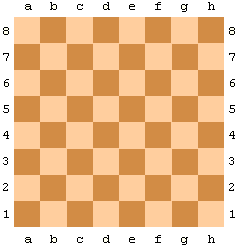
\includegraphics[scale=0.70]{img/tableroajedrez}
	\caption{Tablero}
	\label{contexto:figuratablero1}
\end{figure}

Para la colocación de las piezas, se sitúa el tablero de forma que en la fila más próxima a cada jugador, la casilla de la derecha sea blanca. En la fila más próxima a cada jugador, las torres ocuparán las esquinas, a su lado estarán los caballos, y al lado de estos estarán los alfiles. Las dos casillas centrales estarán ocupadas por la dama, en la casilla de su color, y por el rey en la casilla del color contrario, de forma que ambas figuras estén enfrentadas (en la misma columna) que las del adversario. Los peones irán en la fila inmediatamente siguiente delante de cada una de las figuras. 

En varios problemas de programación competitiva la dimensiones del tablero puede variar enormemente.

\begin{figure}[!h]
	\centering 
	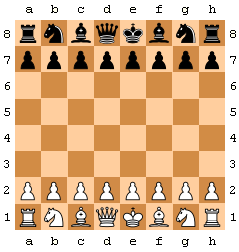
\includegraphics[scale=0.70]{img/posicioni_inicial_ajedrez}
	\caption{Posición incial de las piezas en el tablero}
	\label{contexto:figuratablero}
\end{figure}

\subsection{Rey}

El rey es la pieza más importante del ajedrez, darle jaque mate es el objetivo principal del juego. En caso de que no pueda ser cambiado durante la partida, se la considera una pieza invaluable, sin embargo, algunos autores le atribuyen de dos a cuatro puntos de valor relativo, en una escala de uno a diez, sobre la base de su movilidad, seguridad y el papel activo que juega en el final del juego.

Durante una partida, el rey no puede permanecer bajo la amenaza de piezas enemigas en ningún instante, debe ser colocado de forma segura en el movimiento inmediatamente posterior, en caso de ser atacado. Las reglas de etiqueta en el ajedrez indican que al amenazar al rey del oponente, el atacante puede romper el silencio de la partida y anunciar \emph{¡jaque!} y, en el caso de que el rey no pudiera escapar a la captura, anunciar \emph{¡jaque mate!}. Estos gestos se consideran opcionales según el reglamento del juego.  Cada jugador cuenta con una pieza de este tipo.

\begin{figure}[!h]
	\centering 
	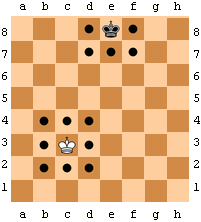
\includegraphics[scale=0.75]{img/movrey}
	\caption{Los escaques marcados indican donde se permite el movimiento.}
	\label{contexto:figurarey}
\end{figure}

\subsection{Dama}

La dama, también conocida como reina, es una pieza mayor del juego de ajedrez, se puede mover vertical, horizontal o diagonalmente cualquier número de escaques. Es la pieza de mayor valor absoluto del juego, valorada con nueve puntos. 

La dama se mueve en línea recta por las filas, columnas y diagonales en el tablero. No puede saltar a sus propias piezas o las adversarias y captura tomando el escaque ocupado por el escaque adversario. Debido a su valor, generalmente se cambia solo por la dama adversaria y su sacrificio, en función de otras piezas, son posiciones que normalmente determinan el resultado de la partida.  Cada jugador cuenta con una pieza de este tipo.

\begin{figure}[!h]
	\centering 
	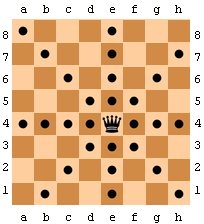
\includegraphics[scale=0.75]{img/movdama}
	\caption{Los escaques marcados indican donde se permite el movimiento.}
	\label{contexto:figuradama}
\end{figure}

\subsection{Torre}

La torre antiguamente llamada \emph{roque}, es una pieza mayor de ajedrez, empleada generalmente en la fase final del juego debido a su valor estratégico y táctico, que ha sido ampliamente estudiada en la literatura ajedrecística. Su valor relativo es de aproximadamente cinco puntos, y puede variar en función de su posición en las filas o columnas abiertas, o formaciones estratégicas como baterías. 

Al comienzo de una partida, cada jugador tiene dos piezas que son dispuestas en las columnas $a$ y $h$, en la primera fila, para las blancas, y en la octava para las negras. 

Se mueve en líneas rectas en las columnas y filas del tablero no pudiendo, sin embargo, saltar piezas adversarias o aliadas y captura al ocupar el escaque dejado por el oponente. Excepcionalmente, si no ha sido movida, se le permite a una de las torres realizar un movimiento especial llamado enroque con el rey, en el cual la torre puede saltar al monarca, ocupando el escaque inmediatamente después de este en el movimiento. 

\begin{figure}[!h]
	\centering 
	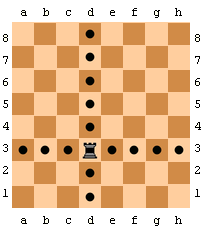
\includegraphics[scale=0.75]{img/movtorre}
	\caption{Los escaques marcados indican donde se permite el movimiento.}
	\label{contexto:figuratorre}
\end{figure}

\subsection{Alfil}

El alfil (antiguamente llamado arfil) es una pieza menor del ajedrez occidental de valor aproximado de tres peones. Se mueve en diagonal, no puede saltar piezas intervinientes, y captura tomando el lugar ocupado por la pieza adversaria. Debido a las características de su movimiento, tiene la deficiencia de la debilidad del color porque su movimiento queda limitado al color del escaque en el que se inicia la partida.

Al comenzar una partida, cada jugador tiene un par de alfiles dispuestos en $c1$ y $f1$ para las blancas y $c8$ y $f8$ para las negras. Su movimiento es oblicuo, moviéndose en línea recta en las diagonales del tablero.

  \begin{figure}[!h]
  	\centering 
  	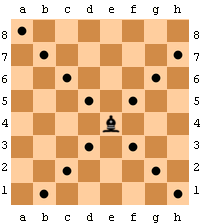
\includegraphics[scale=0.75]{img/movalfil}
  	\caption{Los escaques marcados indican donde se permite el movimiento.}
  	\label{contexto:figuraalfil}
  \end{figure}

\subsection{Caballo}

El caballo es una pieza menor del ajedrez occidental de un valor aproximado de tres peones. Tiene un movimiento semejante a una {\em L} y, a diferencia de otras piezas, puede saltar piezas intermedias. Captura tomando el escaque ocupado por la pieza adversaria. Cada jugador cuenta dos piezas de este tipo.

\begin{figure}[!h]
	\centering 
	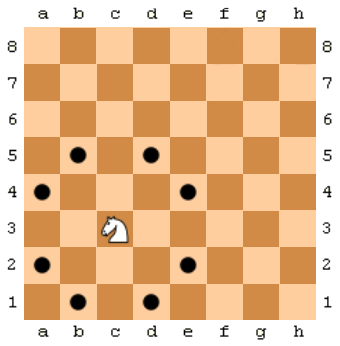
\includegraphics[scale=0.5]{img/movcaballo}
	\caption{Los escaques marcados indican donde se permite el movimiento.}
	\label{contexto:figura1}
\end{figure}

\subsection{Peón}

El peón es una pieza del ajedrez. Al comienzo de una partida, cada jugador tiene ocho peones que están dispuestos en las filas 2 y 7, por delante del resto de piezas. El peón se mueve verticalmente por la columna en la que se encuentra, sin poder retroceder. En el primer movimiento, desde el punto inicial, pueden avanzar dos escaques y, a partir de allí, de uno en uno. 

Para que un peón pueda capturar la pieza debe moverse de su lugar inicial inmediatamente en la fila en diagonal. El peón adversario que avanza dos escaques en su primer movimiento en la columna adyacente y que se sitúa en la misma fila en que se encuentra el peón que va a realizar la captura. Al llegar a la última fila se convierte en cualquier otra pieza, excluyendo el rey, movimiento llamado coronación o promoción; el peón será reemplazado inmediatamente por otra pieza que puede ser caballo, alfil, torre o dama y deberá ser retirado del tablero. La promoción no está limitada a las piezas previamente capturadas, sino que el jugador puede elegir la pieza a la que quiere promocionar, por lo que es posible por ejemplo tener más de una dama en el tablero.

 \begin{figure}[!h]
 	\centering 
 	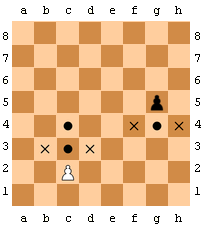
\includegraphics[scale=0.75]{img/movpeon}
 	\caption{Los escaques marcados indican donde se permite el movimiento. Mientras las cruces las posiciones donde puede atacar}
 	\label{contexto:figurapeon}
 \end{figure}